%%!TEX root = diss.tex

\chapter{Collisional Langevin model of bedload sediment velocity distributions}
\label{ch:langevin}
\section{Introduction}

Bedload transport rates show wide and frequent fluctuations which originate from coupling between the fluid and granular phases.
Owing to these fluctuations, measured transport rates often show slow convergence through time \citep{Dhont2018,Turowski2010}, and predicted rates can deviate from measured values by several orders of magnitude \citep{Recking2012,Martin2003}.
These challenges limit numerous ecological and engineering applications that rely on sediment transport predictions \citep{Gaeuman2017,Malmon2005}.

In recent decades, stochastic formulations of the bedload flux have become increasingly popular for their potential to predict the mean transport rates required by applications while also predicting the magnitude of transport fluctuations and quantifying the dependence of measurements on the observation scale (Secs. \ref{sec:birthdeath} and \ref{sec:renewal}).
Recent indications that sediment transport fluctuations might explain longstanding open problems in alluvial channel stability, such as channel width maintenance \citep{Abramian2019,Abramian2020} and bedform initiation \citep{Jerolmack2005,Bohorquez2016} provide additional motivation to develop these stochastic approaches.

One subset of stochastic methods expresses downstream transport rates as a sum over the instantaneous streamwise velocities of all particles in motion within a control volume (Sec. \ref{sec:birthdeath}).
This formulation requires the instantaneous velocity distributions of sediment particles \citep[e.g.][]{Ancey2020a}, yet our understanding of these distributions remains limited.
There is as of yet no consensus on the shape of the bedload velocity distribution, and although the models described in Sec. \ref{sec:langevin} describe some extreme end-member distributions \citep[e.g.][]{Fan2014,Ancey2014}, no models have been developed that describe all experimental observations reported to date \citep{Lajeunesse2010,Fathel2015,Heyman2016,Liu2019,Houssais2012}.
In this chapter, I develop a stochastic model of particle velocities which addresses this shortcoming.

High-speed video experiments have measured different streamwise particle velocity distributions without indicating why one distribution or another appears in a given set of hydraulic and sedimentary conditions.
One set of studies has shown exponential particle velocity distributions \citep{Charru2004,Lajeunesse2010,Roseberry2012,Seizilles2014,Fathel2015,Fathel2016}.
These experiments involve uniformly-sized small sands or glass beads ($0.05-2$mm) in turbulent and subcritical flows, but not always; the experiments of \citet{Lajeunesse2010} were turbulent and supercritical, while the experiments of \citet{Charru2004} and \citet{Seizilles2014} were laminar and likely subcritical.
A second set of studies show Gaussian particle velocity distributions \citep{Ancey2014,Heyman2016,Martin2012}. In these experiments, particles are typically larger ($2-8$mm) uniformly-sized gravels or glass beads, and flows are generally turbulent and supercritical.
Other experiments display velocity distributions that are intermediate between exponential and Gaussian that appear visually more like a Gamma distribution \citep{Houssais2012, Liu2019}.
\citet{Houssais2012} used a bimodal distribution of glass beads with diameters $0.7$mm and $2.2$mm in turbulent and supercritical flow conditions, while \citet{Liu2019} used sand having median diameter $1.1$mm in turbulent and subcritical flow.
From this experimental record, the velocity distribution shape apparently does not consistently relate to the flow conditions.
There is however a loose trend within the particle size.
Smaller particles tend to show more exponential-like distributions \citep[e.g.][]{Fathel2015}, while larger ones show Gaussian distributions \citep[e.g.][]{Heyman2016}. This summary suggests that streamwise bedload velocity distributions could be controlled by the particle size.

Existing models of streamwise bedload velocities can be divided into computational and stochastic physics categories.
Computational models numerically integrate some approximate coupled dynamics for individual grains and the fluid, generally modeling particles as spheres interacting through repulsive forces and numerically integrating the Navier-Stokes equations (or some approximation of them) to describe the flow forces on grains.
When streamwise particle velocities have been analyzed in such simulations, they show exponential tails \citep{Gonzalez2017,Furbish2013} that agree with one subset of the experimental data.

Stochastic models have incorporated fluctuating driving and resisting terms into Newtonian equations of individual grains to develop Langevin-like descriptions of bedload particle motions (Sec. \ref{sec:langevin}). \citet{Fan2014} represented turbulent drag as Gaussian white noise and included a static Coulomb friction term to model particle-bed collisions, while \citet{Ancey2014} applied an Ornstein-Uhlenbeck process which combines the fluid and driving forces into a simplified velocity-dependent force, again modeling fluctuations with Gaussian white noise.
Each of these models derives one end-member distribution from among the range of distributions reported in experiments.
A physical description for the full range of experimentally-observed bedload velocity distributions remains an elusive target.

In this chapter I explore the possibility that the particle velocity distribution is controlled by momentum dissipation from particle-bed collisions by incorporating ideas from the physics of granular media.
A major paradigm in granular dynamics is to describe particles as a continuum or ``granular liquid" having an effective rheology \citep[e.g.][]{Jenkins1998,Andreotti2013}, but as discussed in Ch. \ref{ch:Introduction} such a continuum assumption is unlikely to be satisfied for weak bedload transport conditions. 

Instead, particles in these conditions are better characterized as a rarefied granular gas \citep[e.g.][]{Furbish2021}. 
In granular gases, dissipative collisions are known to cause departures toward an exponential velocity distribution from the Gaussian form expected for perfectly elastic collisions \citep{Brilliantov2004}.
Gas theory formulates particle-particle collisions as a nonlocal integral within the master equation for the probability distribution of particle velocity called the Boltzmann equation \citep{Landau1969,Chapman1970,Brilliantov2004}.
Collisions in these models involve episodic kicks to the particle momenta at random times, usually parameterized by billiard ball-like models of the underlying rigid body dynamics \citep[e.g.][]{Brach1989}.
Such episodic forcing is distinct from the smooth friction terms included in the current stochastic models describing bedload particle velocities.

I develop in this chapter an improved model for sediment grains in transport which replaces the smooth friction terms of earlier models by episodic particle-bed collisions.
I present the model and explain its key assumptions in Sec. \ref{sec:langmodel}. Then I explain the analytical solution of the model and other major results in Sec. \ref{sec:langresults}. Finally I discuss the implications of these results, summarize key findings, and suggest ideas for further research in Secs. \ref{sec:langdiscussion} and \ref{sec:langconclusion}.


\section{Mechanistic description of particle velocities}
\label{sec:langmodel}

Fig. \ref{fig:fig1} indicates the configuration of the model in this chapter.
Nearly spherical particles of diameter $d$ and mass $m$ move as bedload over a granular bed.
The flow is just strong enough to drive grains into the rarefied transport often typical in gravel-bed rivers \citep[e.g.][]{Ashworth1989, Warburton1992}. Particles saltate downstream through a sequence of particle-bed collisions, and moving particles collide often with stationary particles but rarely with other moving particles \citep[cf.][]{Williams2021}.

Particles respond to turbulent flow forces and episodic particle-bed collision forces. In contrast to the computational physics approach, I do not aim to characterize the exact timeseries of the forces on an individual particle. Instead, I model the ensemble of possible force timeseries that particles could conceivably experience. Each force timeseries realization implies a different velocity timeseries $u(t)$ in the downstream direction.
The objective is to calculate the probability distribution $P(u,t)$ of this downstream velocity by averaging over the ensemble of forces.

The description of bedload particle velocity fluctuations will be more detailed than the simple white noise model Ch. \ref{ch:flux}, but alternation between motion and rest will be neglected, meaning the model of this chapter is only applicable to moving particles.
In analyzing the velocities of moving particles, I include the most realistic particle-bed collision and fluid forces possible while still allowing for analytical solutions.

\subsection{Episodic collision forces}
Collisions between bedload particles dissipate translational momentum, partly by converting it to vertical, lateral, or angular momentum, partly by deforming particles and the bed and generating heat \citep{Schmeeckle2014,Williams2021}, and partly by pressurizing the fluid between approaching particles \citep{Joseph2001,Schmeeckle2001}. 
The microscopic details of particle-particle collisions have been thoroughly studied \citep{Brach1989, Lorenz1997,Montaine2011}, although in bedload transport the coefficient of restitution may be less relevant than other factors such as collision geometry and bed deformation \citep{Pahtz2021}. Here, I introduce a simple elasticity parameter $\varepsilon$ as a first attempt at modeling dissipation by episodic collisions, as indicated in Fig. \ref{fig:fig1}. This elasticity characterizes the fraction of downstream momentum lost in a collision. If the streamwise velocity just prior to a collision is $u$, just after the collision it becomes $\varepsilon u$. The elasticity ranges from $\varepsilon=0$, representing a completely inelastic collision, to $\varepsilon=1$, representing a completely elastic collision.
\begin{figure}
	\centerline{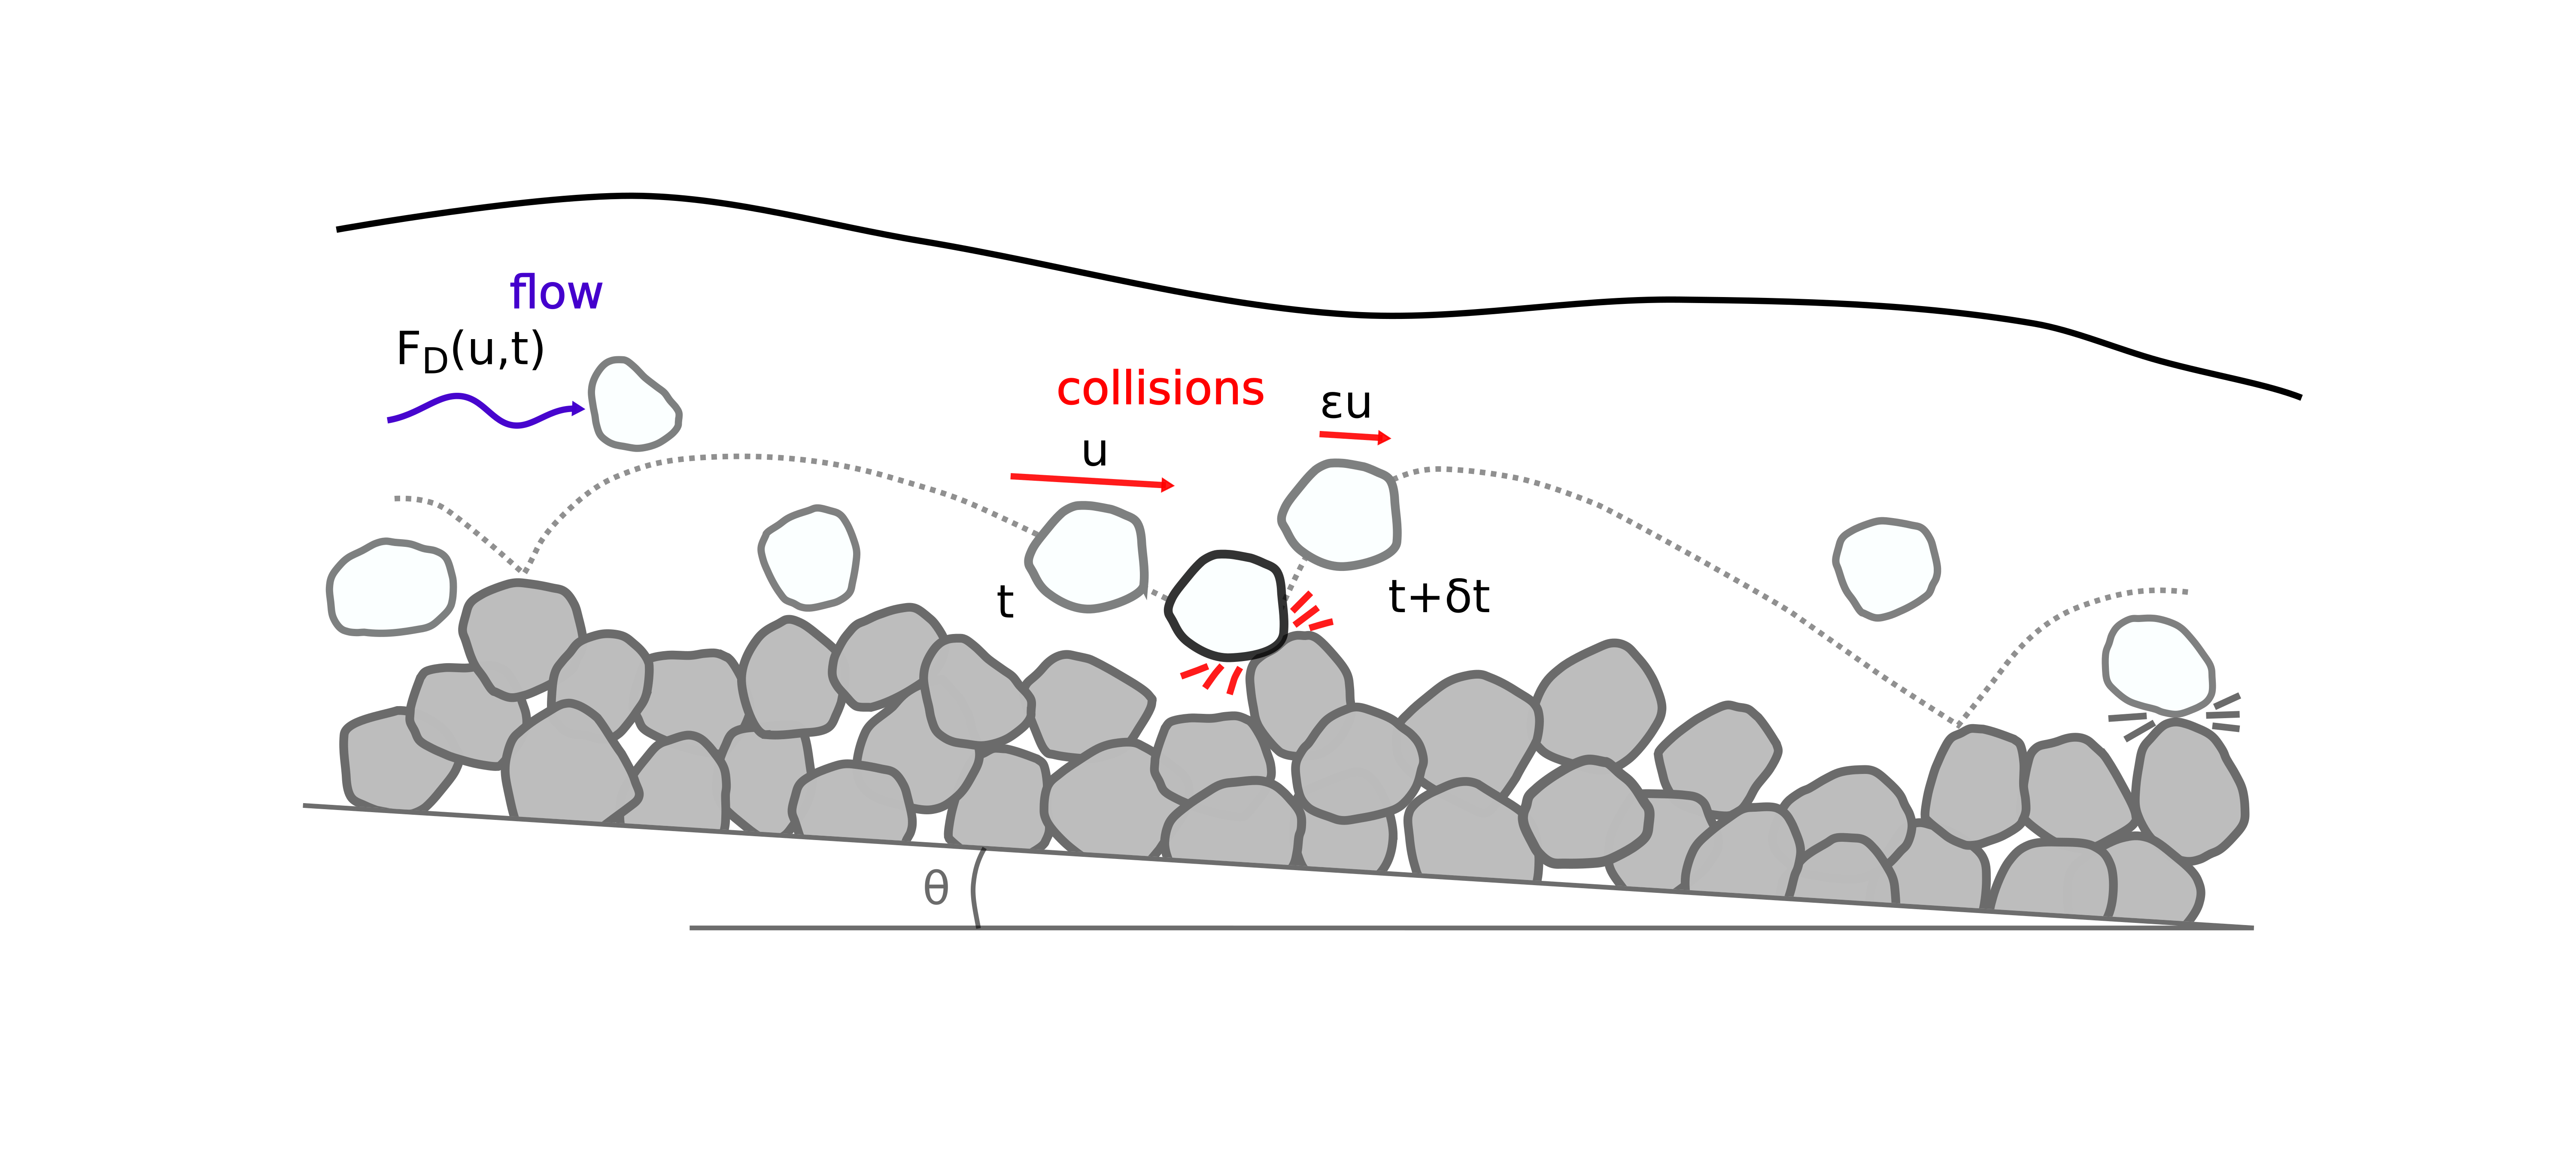
\includegraphics{./figures/ch5/Fig1Concept.png}}
	\caption{Rarefied sediment transport involves turbulent fluid drag and episodic particle-bed collisions. In the collision model developed in this chapter, pre-collisional streamwise velocities $u$ are transformed instantaneously to post-collisional velocities $\ve$. The parameter $\ve$ is an ``elasticity" with $0\leq \ve \leq 1$.}
	\label{fig:fig1}
\end{figure}

Since the elasticity combines effects of particle shape and collision geometry and should vary from one collision to the next, the elasticity $\varepsilon$ is interpreted as a random variable, characterized by a statistical distribution $\rho(\varepsilon)$.
Some granular gas models have also included random elasticity \citep[e.g.][]{Serero2015}, but this topic has not been completely explored in the literature.

Assuming that the average number of collisions per unit time is $\nu$ (the collision rate) and that the time intervals between subsequent particle-bed collisions are exponentially distributed \citep[e.g.][]{Gordon1972}, the collision force in the downstream direction can be written as a Poisson pulse noise (Sec. \ref{sec:einflux}):
\be F_C(u,t) = - m u \sum_{k=1}^{N_\nu(t)}(1-\varepsilon_k)\delta(t-\tau_k). \label{eq:col} \ee
Here, $N_\nu(t)$ is the number of collisions in time $t$ (a Poisson random variable), the $\tau_k$ ($k=1,2,\dots$) are times at which collisions occur, and the $\varepsilon_k$ are the elasticity coefficients, drawn from the distribution $\rho(\varepsilon)$ characterizing the fraction of momentum lost in each particle-bed collision.
The time intervals $\Delta \tau = \tau_k-\tau_{k-1}$ between collisions are distributed as $P(\Delta \tau) = \nu \exp(-\nu\Delta \tau),$ so the number of collisions $n=N_\nu(t)$ in time $t$ is distributed as $P(n) = (\nu t)^n\exp(-\nu t)/n! .$
This collision force is a sequence of random impulses which are proportional to the pre-collisional streamwise momenta. This collision model should be adequate when the contact times between moving and resting particles are small compared to the times between collisions. These conditions should be satisfied for typical saltation trajectories as in Fig. \ref{fig:fig1}.

\subsection{Turbulent fluid forces}

Fluid forces on coarse particles are parameterized by the particle Reynolds number $\Rey_p = V d/\lambda$, involving the particle size $d$, slip velocity $V$ between particle and fluid, and kinematic viscosity $\lambda$.
These forces have been calculated from the Navier-Stokes equations for spherical particles at small (or vanishing) $\Rey_p$ and include drag, virtual mass, buoyancy, fluid pressure gradient, Basset history integral, Saffman lift, and Magnus lift terms \citep{Hjelmfelt1966, Maxey1983, Auton1987}.
At realistic $\Rey_p$, analytical results for the fluid forces on a particle remain inaccessible, so it is standard practice to introduce empirical corrections to the small $\Rey_p$ formulas \citep[e.g.][]{Clift1978,Schmeeckle2007}.

Our understanding of the fluid forces remains incomplete.
Existing formulas were derived in the absence of boundaries, so it is unclear how these formulas should be modified near the bed.
Even ignoring this complication, the added mass and Basset forces are difficult to compute and therefore impractical to include in analytical models.
These challenges require us to adopt the most complex expressions of the fluid forces that are compatible with our modeling goals \citep[e.g.][]{Michaelides1997,Armenio2001}.
From this same requirement, a majority of bedload transport models include fluid drag (and possibly pressure gradient) terms as the only force(s) driving the downstream movement of bedload particles \citep{Ancey2014,Fan2014,Schmeeckle2014,Gonzalez2017,Elghannay2017}.

The downstream drag force with an $\Rey_p$ correction is usually written 
\be F_D = \frac{\pi}{8} \rho_f d^2 C_D(\Rey_p) |V|V, \label{eq:draggy}\ee
where $\rho_f$ is the fluid density, $d$ is the particle diameter, $C_D(\Rey_p)$ is an empirical drag coefficient, and $V = U-u$ is the slip velocity calculated as the difference of fluid ($U$) and particle ($u$) velocities \citep{Coleman1967, Schmeeckle2007, Dwivedi2012}.
Experiments on stationary particles indicate that drag forces fluctuate rapidly and lie on wide Gaussian-like distributions \citep{Hofland2006,Schmeeckle2007,Dwivedi2010,Celik2014}.
Drag forces on moving particles have not been experimentally measured, but even in globally steady flow conditions, slip velocities are expected to fluctuate due to particle acceleration, fluid turbulence, passage of other moving particles, and vertical movement of particles within the flow profile.
The nonlinearity in Eq. \ref{eq:draggy} will amplify slip velocity fluctuations, generating large and erratic drag force variations that only add to the undetermined contributions of the neglected fluid forces.

Here I assume with earlier computational \citep{Schmeeckle2014,Gonzalez2017,Elghannay2017} and analytical \citep[e.g.][]{Ancey2014,Fan2014} models of bedload transport that fluid drag is the primary force driving sediment particles downstream. I further assume with \citet{Fan2014} and \citet{Ancey2014} that the fluctuating component of this force can be represented by a Gaussian white noise.
This latter assumption is justified insofar as drag forces fluctuate rapidly compared to the inertial response times of particles and the timescales over which particles change height within the flow profile.
Defining $\bar{C}_D$ as the empirical drag coefficient evaluated at $\bar{V}$ and $\xi(t)$ as a Gaussian white noise of mean $0$ and variance $1$ \citep[e.g.][]{Gardiner1983}, the fluid drag force considered in this chapter is
\be F_D(t) = \Gamma + \sqrt{2 D } \eta(t), \label{eq:drag}\ee
where $\Gamma = \frac{\pi}{8}
\rho_f d^2 \bar{C}_D \bar{V}^2$ is the steady component of the drag.
Although this representation of the fluid forces is a simplified approximation, it is similar to the representations used in earlier stochastic models in that it has no dependence on the vertical structure of the flow \citep[e.g.][]{Fan2014,Ancey2014}. This level of simplification is required for an analytically tractable model of bedload particle velocities \citep[e.g.][]{Michaelides1997}.

\subsection{Langevin equation for collisional bedload transport}

With the above forces, the Langevin equation $m\dot{u}(t) = F_D(t) + F_C(t)$ for the sediment dynamics in the downstream direction becomes
\be m \dot{u}(t) = \Gamma + \sqrt{2D}\eta(t) - m u(t) \xi_{\nu, \ve}(t). \label{eq:langevin} \ee
This equation replaces the steady friction terms of earlier models with an episodic term, designed to provide a more realistic representation of particle-bed collisions.
Mathematically, Eq. \ref{eq:langevin} is a Langevin-like equation representing a jump-diffusion process \citep{Daly2006} with multiplicative Poisson noise \citep{Dubkov2016,Denisov2009}. 
Collisions introduce velocity jumps while turbulence generates velocity diffusion. The collision term is multiplicative in the sense that $u$ multiplies the Poisson noise $\xi_{\nu,\ve}(t)$.

Models like Eq. \ref{eq:langevin} have long been studied in the stochastic physics literature \citep{Hanggi1978,VanDenBroeck1983}, but solving such equations remains extremely challenging \citep{Daly2010,Mau2014,Dubkov2019}.
One issue is that multiplicative white noises imply the prescription dilemma of stochastic calculus \citep{Risken1989,Gardiner1983}, meaning Eq. \ref{eq:langevin} is not defined without further specifying an integration rule \citep{Suweis2011}.
Here, the It\^{o} interpretation (lower endpoint integration rule) is the physical choice the energy dissipated by collisions depends strictly on pre-collisional velocities, not post-collisional \citep[e.g.][]{Gardiner1983}.
Given this integration rule, the remaining issues are to obtain the master equation characterizing the ensemble of velocities defined by Eq. \ref{eq:langevin}, and then to solve this equation for the velocity distribution $P(u,t)$.

\subsection{Master equation and particle-bed collision integral}

The equation governing the streamwise velocity distribution $P(u,t)$ is derived in the appendix Sec. \ref{sec:langmasterderiv} with a limiting procedure, providing
\be \nu^{-1}\partial_t P(u,t) = - \tilde{\Gamma} \partial_u P(u,t) + \tilde{D} \partial_u^2 P(u,t) + I_c(u,t). \label{eq:master} \ee
The parameters $\tilde{\Gamma} = \Gamma/(\nu m)$ and $\tilde{D} = D/(\nu m)$ scale the steady and fluctuating components of the fluid force against the collision rate $\nu$. The term
\be I_c(u,t) = - P(u,t) + \int_0^1 \frac{d\ve}{\ve}P\big(\frac{u}{\ve},t \big) \rho(\ve) \label{eq:colint} \ee
is a ``collision integral" term representing particle-bed collisions.

Eq. \ref{eq:master} is a nonlocal extension of the Fokker-Planck equation used in earlier bedload models \citep{Fan2014,Ancey2014}. 
Nonlocality is introduced by the collision integral of Eq. \ref{eq:colint} which transfers probability from higher pre-collisional velocities $u/\varepsilon$ to lower post-collisional velocities $u$.
This term is analogous to the collision integral within the Boltzmann equation of kinetic theory \citep{Duderstadt1979, Brilliantov2004}. Physically, it corresponds to binary collisions between particles having different masses and random restitution coefficients \citep[cf.][]{Serero2015} in the limit that the mass of one particle (here, the particle resting on the bed) diverges to infinity.
Mathematically, the collision integral represents the probability distribution of the product between the elasticity $\varepsilon$ and the downstream momentum $(p = m u)$, considering them as uncorrelated random variables \citep[cf.][]{Feller1968}.


Owing to its nonlocality, Eq. \ref{eq:master} does not admit analytical solutions as is, so further approximation is necessary.
To make progress, I assume the distribution of elasticity $\rho(\varepsilon)$ is sharply peaked at some most common (mode) value $\varepsilon'$ to allow for a Kramers-Moyal type expansion of the particle-bed collision integral \citep[e.g.][]{Gardiner1983}.
Such a mode value in the collision elasticity distribution is present in experiments on rigid body collisions \citep{Glielmo2014}.
For particle-bed collisions of bedload, a modal elasticity is also expected since experiments indicate a most common collision geometry \citep[e.g.][]{Gordon1972,Martin2013}.

Expanding all terms in the integrand except $\rho(\varepsilon)$ provides
\be I_c(u,t) = -P(u,t) + \frac{1}{\varepsilon'}P\big(\frac{u}{\ve'},t \big) + \sum_{k=1}^\infty \frac{\alpha_k }{k!}(\ve - \ve')^k \Big[\frac{1}{\ve}P\big(\frac{u}{\ve}\big)\Big]^{(k)}\Big|_{\ve=\ve'},\label{eq:expansion}\ee
where the $\alpha_k = \int_0^1 d\ve \rho(\ve) (\ve-\ve')^k $ are the central moments of $\ve$ around the modal elasticity $\ve'$ and the superscript $(k)$ denotes the $k$th derivative.

In what follows, I drop all but the first two terms in this expansion to obtain the leading order contribution of particle-bed collisions to the velocity distribution.
Higher orders could always be included later by perturbation theory \citep{Morse1953a}.
I solve the resulting approximate equation in steady-state, when $\partial P(u,t)/\partial t = 0$. Eq. \ref{eq:master} indicates that this solution will be a good approximation to the time-dependent problem when particle motions generally survive multiple collisions ($t\gg \nu^{-1}$).

\section{Results}
\label{sec:langresults}

\subsection{Derivation of the bedload velocity distribution}
\label{sec:langsolution}
Hereafter I drop the prime on the most common streamwise restitution coefficient $\ve'$.
With the truncation to two terms, Eq. \ref{eq:master} gives 
\be 0 = -\tilde{\Gamma}\partial_u P(u) + \tilde{D}\partial_u^2 P(u) -P(u) + \frac{1}{\ve} P\big(\frac{u}{\ve}\big),\label{eq:governer} \ee
which is an advanced functional differential equation. This equation is ``functional" in the sense that it is nonlocal in velocity due to the last term on the right hand side, and it is ``advanced" in that $u/\ve$ is advanced beyond the argument $u$ involved in the rest of this equation (since $0<\ve<1$).
Such equations have seen some attention in the mathematics literature, where they are sometimes called pantograph equations \citep{Hall1989, Kim1998,Zaidi2015}.

In the appendix Sec. \ref{sec:langsteadyderiv} Eq. \ref{eq:governer} is solved with Laplace transforms, providing
\begin{multline} P(u) = \frac{\theta(-u)}{K_+}\sum_{l=0}^\infty \frac{\ve^{-l}e^{\lambda_+\ve^{-l}u}}{\prod_{m=1}^l(-\tilde{D} \lambda_+^2 \ve^{-2m} + \tilde{\Gamma} \lambda_+ \ve^{-m} + 1) } 
	\\+ \frac{\theta(u)}{K_-}\sum_{l=0}^\infty \frac{\ve^{-l}e^{\lambda_-\ve^{-l}u}}{\prod_{m=1}^l(- \tilde{D} \lambda_-^2 \ve^{-2m} + \tilde{\Gamma} \lambda_- \ve^{-m} + 1) } \label{eq:steadystate}. \end{multline}
The factors $\lambda_\pm$ are defined in appendix Eq. \ref{eq:lambdas}. They are proportional to $\tilde{\Gamma}/\tilde{D}$. 
The normalization factors $K_\pm$ are 
\be K_\pm = \tilde{D}(\lambda_+-\lambda_-)\prod_{l=1}^\infty (- \tilde{D}\lambda_\pm^2 \ve^{2l} +\tilde{\Gamma} \lambda_\pm \ve^{l} + 1). \ee
Although this velocity distribution has a complex mathematical structure, one can verify that this is a normalized probability distribution ($\int du P(u) = 1$) which has very simple limiting behaviors as the mode elasticity $\ve$ approaches fully elastic ($\ve=1$) and inelastic ($\ve = 0$) values.

It is possible to derive the moments of this probability distribution by multiplying Eq. \ref{eq:governer} by $u$, integrating, and then solving the resulting moment evolution equations \citep[e.g.][]{Cox1965}.
These calculations are provided in the appendix Sec. \ref{sec:langmoments}, where the mean bedload velocity is derived as
\be \langle u \rangle = \frac{\Gamma}{\nu(1-\ve)} = \frac{\tilde{\Gamma}}{1-\ve}. \label{eq:meanu}\ee
This result scales linearly with the mean fluid drag and nonlinearly with the rate and typical elasticity of collisions, indicating a strong influence of particle collisions on bedload velocities.
The second moment is
\be \langle u^2 \rangle = 2 \frac{\tilde{D} + \tilde{\Gamma} \langle u \rangle}{1-\ve^2}, \ee
leading to the velocity variance ($\sigma_u^2 = \bra u^2 \ket - \bra u \ket ^2 $)
\be \sigma_u^2 = \frac{2 \tilde{D}+ \tilde{\Gamma}^2}{1-\ve^2}. \label{eq:varu}\ee
This result demonstrates that within the model, velocity fluctuations originate from both the steady and fluctuating components of the flow forces, yet the variance is linear in these factors and is therefore relatively insensitive to the fluid flow.
This is consistent with the similarities apparent between viscous and turbulent flow experiments \citep[e.g.][]{Charru2004,Lajeunesse2010}.
In contrast, particle velocity fluctuations in Eq. \ref{eq:varu} depend sharply on the parameters representing particle-bed collisions, suggesting collisions could be the leading control on particle velocity fluctuations.

Fig. \ref{fig:fig2} depicts the velocity characteristics of particles for different realizations of the fluid and collisional forces.
\begin{figure}
	\centerline{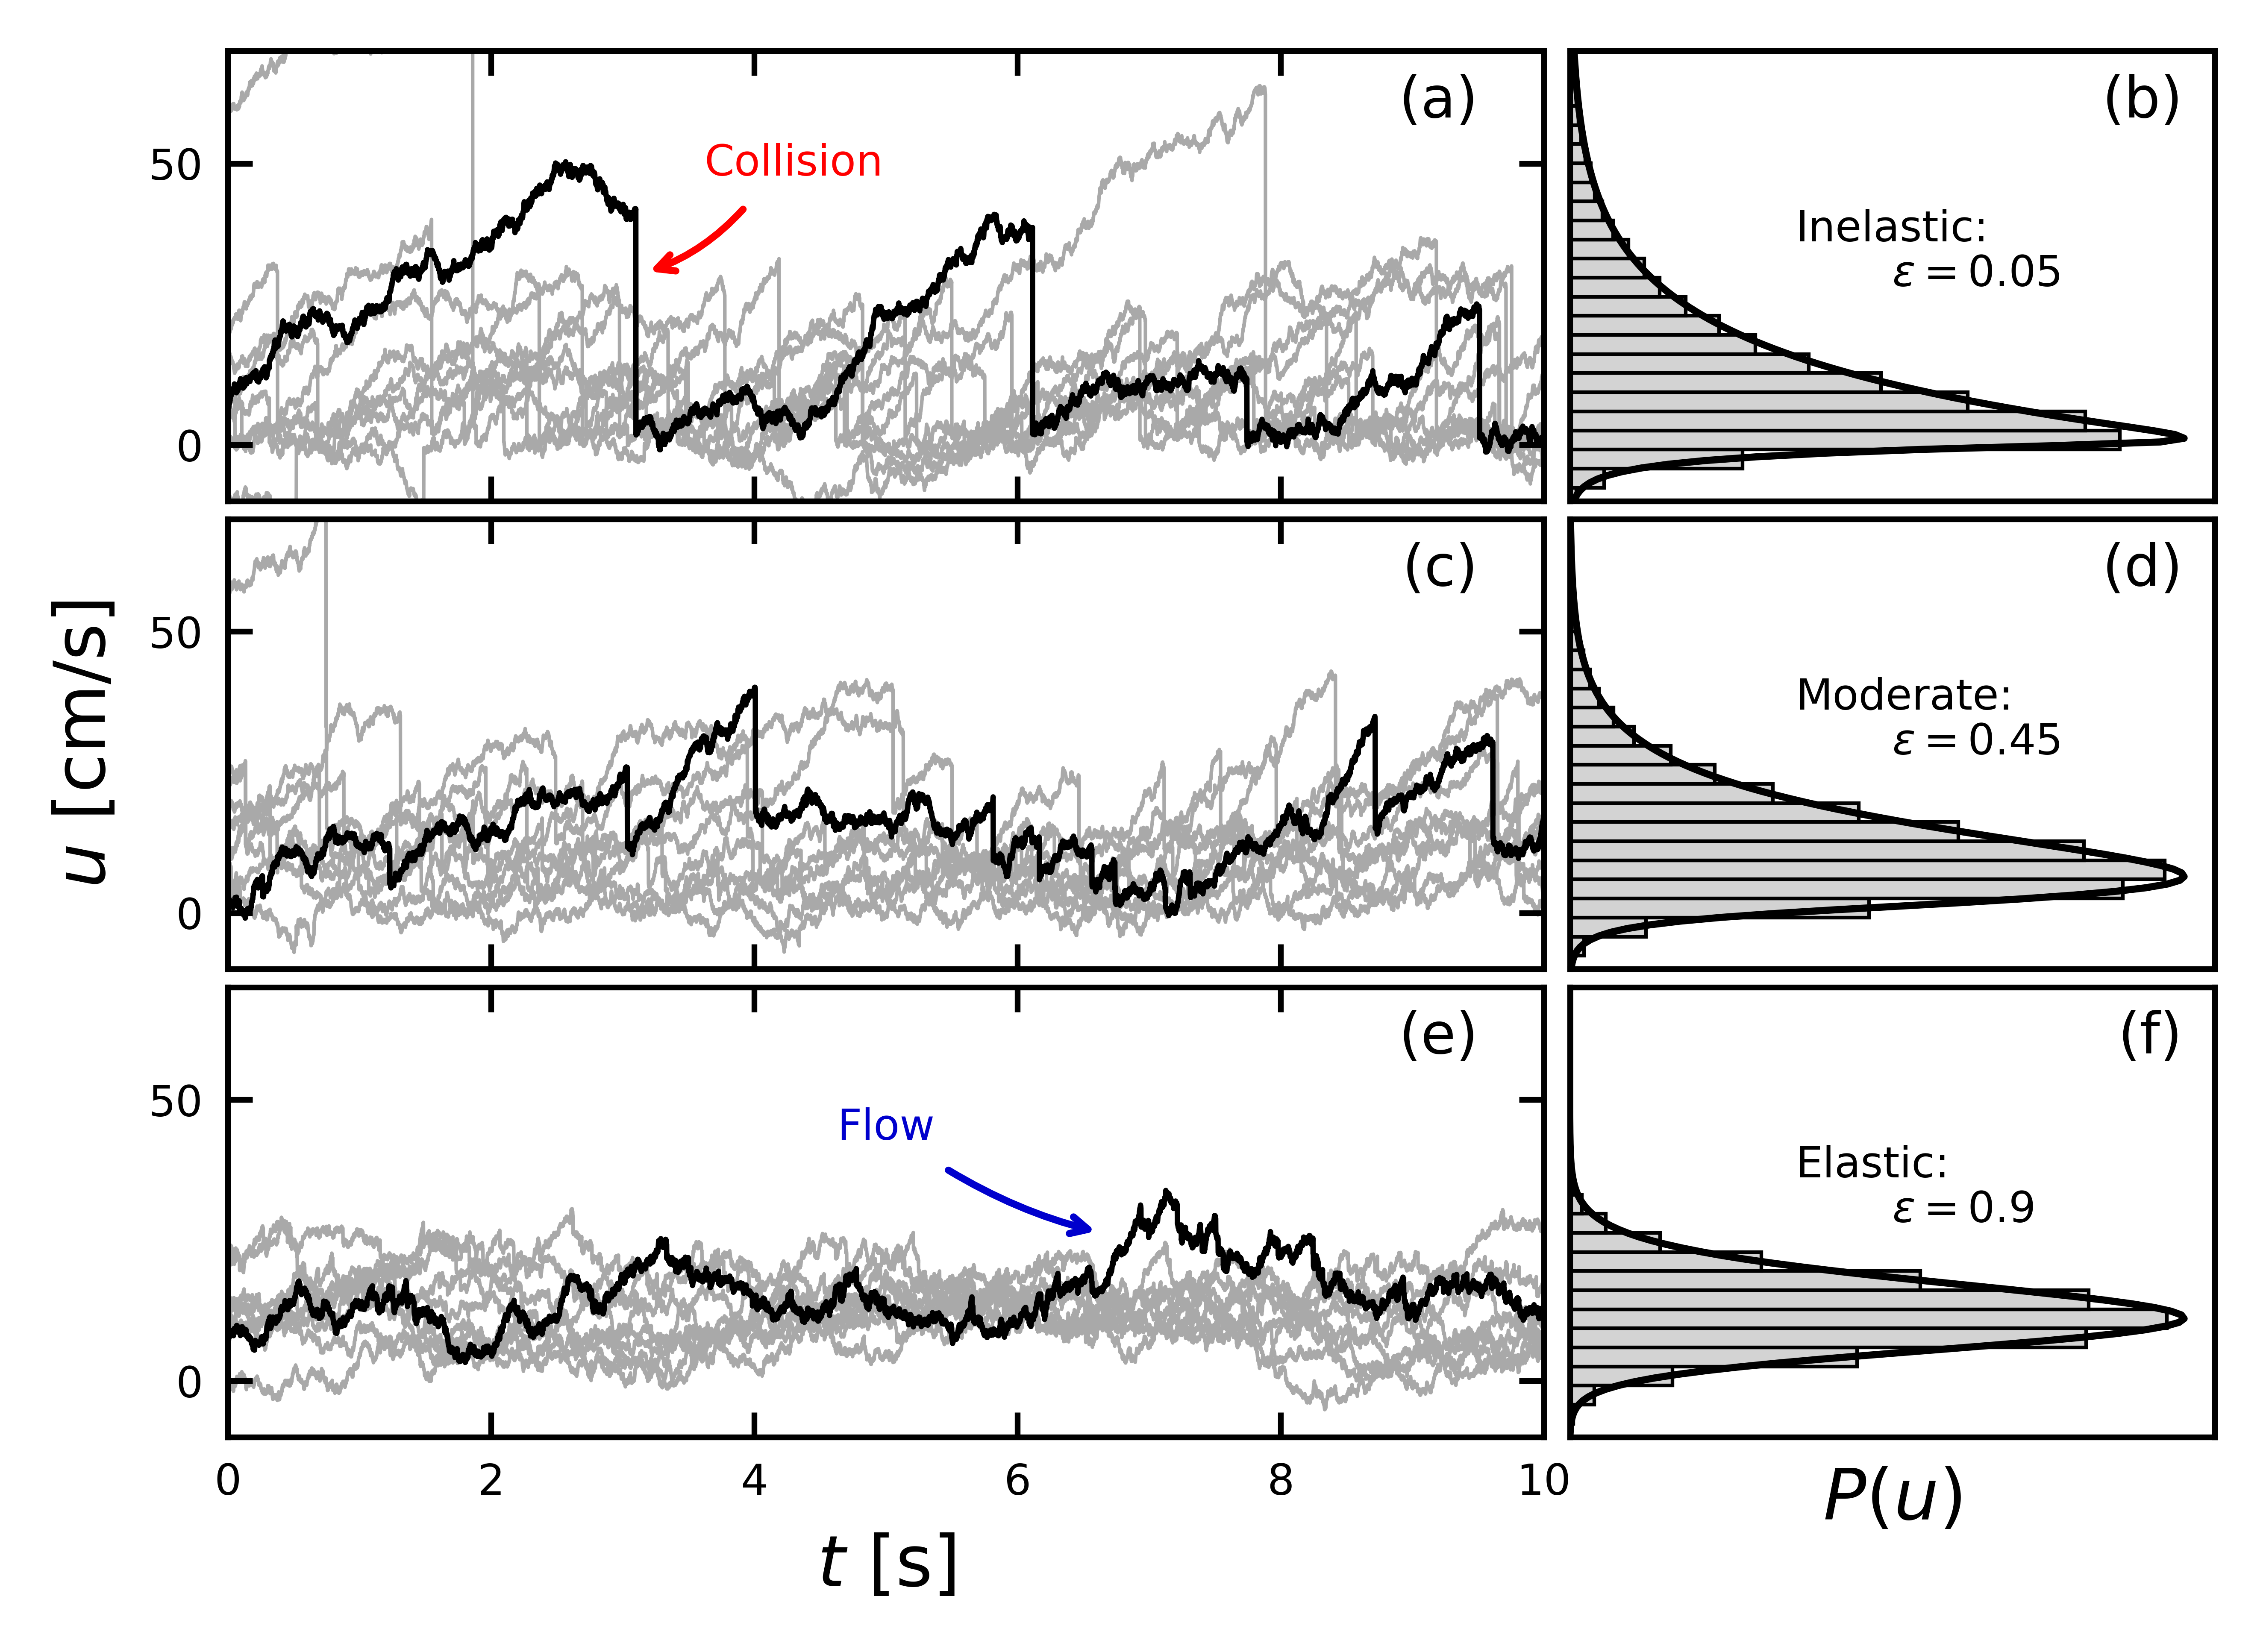
\includegraphics{./figures/ch5/Fig2pdfs.png}}
	\caption{Left and right panels are paired. Left panels show velocity realizations as gray traces. Velocities are calculated from Monte Carlo simulations. Individual realizations are singled out as black traces. Particle-bed collisions imply sudden downward-velocity jumps. Flow forces generate fluctuating positive accelerations between collisions. Right panels show simulated histograms of particle velocities and exact solutions from Eq. \ref{eq:steadystate}. As the elasticity $\ve$ varies, the particle velocity distributions interpolate between exponential (inelastic) and Gaussian (elastic) forms.}
	\label{fig:fig2}
\end{figure}
Fig. \ref{fig:fig2} reveals an apparent transition from exponential to Gaussian-like velocity distributions as collisions vary from more inelastic ($\ve \rightarrow 0$) to more elastic ($\ve \rightarrow 1$). In between, the full distribution Eq. \ref{eq:steadystate} resembles a Gamma distribution, although it is represented by Eq. \ref{eq:steadystate}, not a Gamma distribution.


\subsection{Exponential and Gaussian regimes: Limits to earlier work}
\label{sec:langmodelcomparison}

In fact, the apparent transition from exponential to Gaussian in Fig. \ref{fig:fig2} can be demonstrated analytically from Eq. \ref{eq:steadystate}. Despite its complex appearance, simple Gaussian and exponential forms derive from this equation as exact mathematical limits.
When particle-bed collisions are completely inelastic ($\ve = 0$), Eq. \ref{eq:steadystate} becomes an exponential distribution, and when they are completely elastic ($\ve = 1$), Eq. \ref{eq:steadystate} becomes Gaussian.
Fig. \ref{fig:fig3} demonstrates in detail the approach of the distribution toward these limits.
\begin{figure}
	\centerline{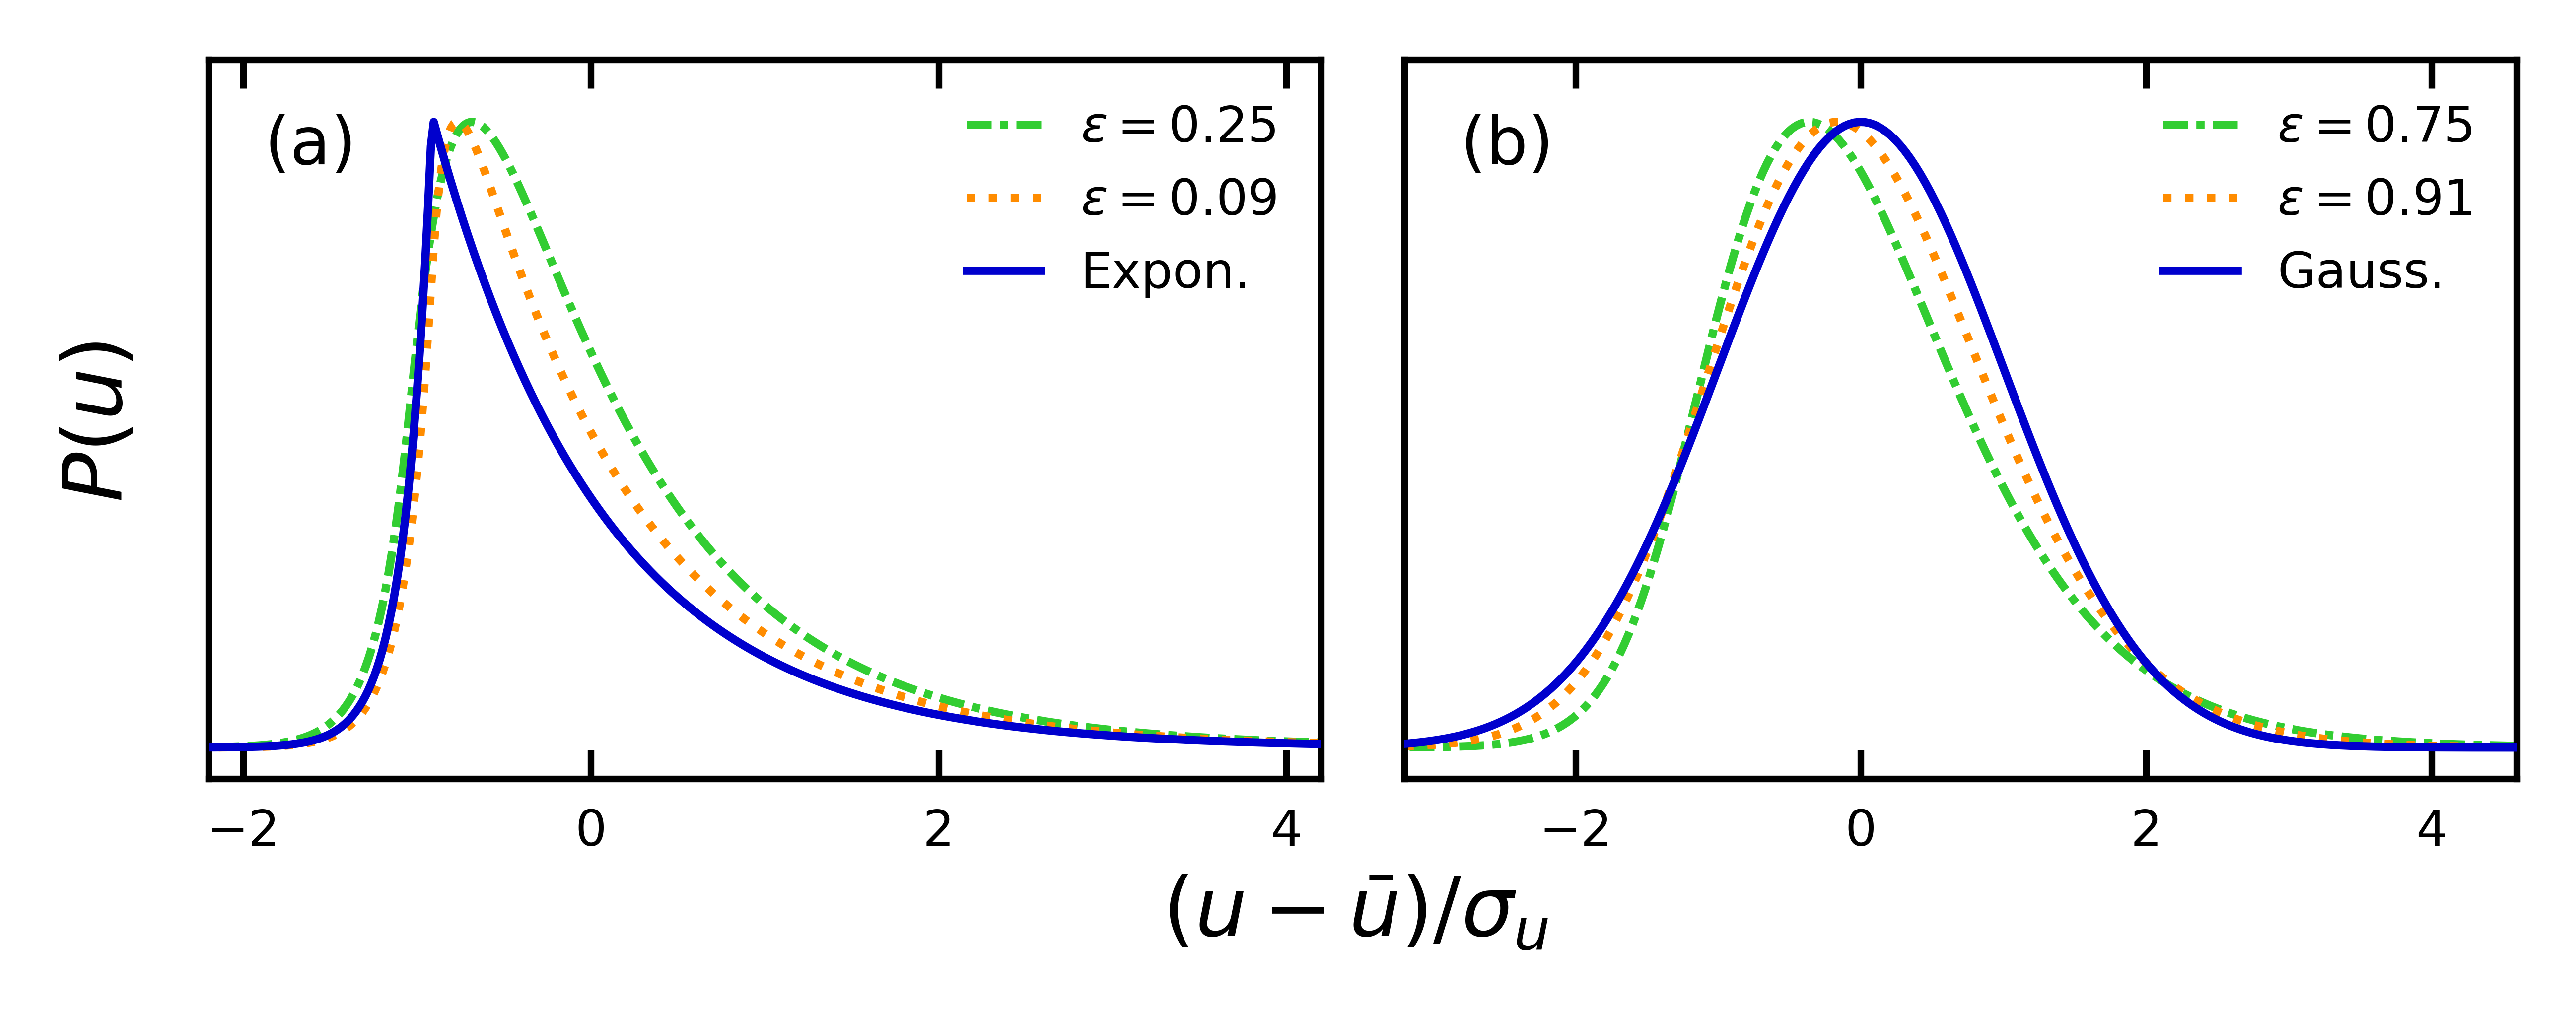
\includegraphics{./figures/ch5/Fig3asymptotic.png}}
	\caption{The particle velocity distribution approaches an exponential distribution in panel (a) as particle-bed collisions become extremely elastic ($\ve \rightarrow 1$), and it approaches a Gaussian in panel (b) as they become extremely inelastic ($\ve \rightarrow 0$). On the abscissa, the mean sediment velocity is standardized by its mean $\bar{u}$ and standard deviation $\sigma_u$. }
	\label{fig:fig3}
\end{figure}

The exponential limit of Eq. \ref{eq:steadystate} as $\ve \rightarrow 0$ is easy to see. Taking $\ve \rightarrow 0 $ in Eq. \ref{eq:steadystate}, all terms in the series except for the one at $l=0$ become exponentially small, leaving behind the same two-sided exponential distribution derived by \cite{Fan2014} up to differences in notation:
\be P(u) = \frac{\tilde{D}}{\sqrt{\tilde{\Gamma}^2 + 4 \tilde{D}}}e^{\frac{\tilde{\Gamma} u }{2 \tilde{D}} - \frac{\sqrt{\tilde{\Gamma}^2 + 4 \tilde{D}}|u|}{2\tilde{D}}}. \ee
Thus, for bedload transport conditions with typically very inelastic particle-bed collisions, we can expect exponential-like velocities and large deviations from a Gaussian behavior.

The Gaussian limit as $\ve \rightarrow 1$ of Eq. \ref{eq:steadystate} is more difficult to evaluate. The challenge is that the statistical moments (Eqs. \ref{eq:meanu} and \ref{eq:varu}) diverge at the same time as the denominator factors of the distribution Eq. \ref{eq:steadystate}. In the appendix Sec. \ref{sec:langextremes} I return instead to the original equation \ref{eq:governer} to evaluate the completely elastic limit, obtaining
\be P(u) = \frac{1}{\sqrt{2\pi\sigma_u^2}}e^{-\frac{(u-\bar{u})^2}{2\sigma_u^2}}. \label{eq:gaussian}\ee
This result is identical to the velocity distribution derived by \citet{Ancey2014}, up to notation.

\subsection{Comparison with experimental data}
\label{sec:langexperimentcomparison}

A variety of velocity distributions have been observed in bedload transport experiments, ranging from exponential to Gaussian in shape. 
This section compares Eq. \ref{eq:steadystate} with the results of six different experiments.
Comparing Eq. \ref{eq:steadystate} with experimental data requires values for the steady component of the drag force $\Gamma$, the particle mass $m$, the magnitude of turbulent drag fluctuations $D$, the rate of particle-bed collisions $\nu$, and the modal elasticity of collisions $\varepsilon$.

In each case, the particle mass is computed from experimental parameters assuming spherical sediment as $m = \pi \rho_s d^3/6$, where $\rho_s$ is the sediment density and $d$ is the particle diameter.
The characteristic slip velocity entering the steady component of the drag force in Eq. \ref{eq:drag} is not obviously related to any one velocity scale of the fluid flow. It should really be calculated as an average over different particle heights, particle velocities, and fluid velocities within the flow profile. For lack of a better option I simply assume the typical slip velocity scales with the shear velocity of the flow, as it would for a small particle resting on the bed. Using this assumption, the steady component of the drag force is estimated as
\be \Gamma =  \frac{\pi}{8}\rho C_D(\Rey_p) d^2 u_\ast^2,\ee
where $\rho$ is the fluid density and $C_D(\Rey_p)$ is the drag coefficient, given as \citep{Clift1978,Gonzalez2017}
\be C_D = \frac{24}{\Rey_p}( 1 + 0.194 \Rey_p^{0.631}). \ee
Particle Reynolds numbers are estimated using the shear velocity: $\Rey_p= u_\ast d/\lambda$. 
The magnitude $D$ of turbulent fluctuations, collision elasticity $\ve$, and collision rate $\nu$ are treated as calibration parameters and are tuned to provide best fit between the distribution \ref{eq:steadystate} and the experimental data.

The parameters for each experiment and the best-fit calibration parameters are collected in Tab. \ref{tab:calib}, while the results of fitting the model to the available experimental data are shown in Fig. \ref{fig:fig4ch5}.
\begin{table}
	\begin{center}
		\def~{\hphantom{0}}
		\begin{tabular}{l|ccccccc}
			Experiment & $d$ [$mm$] & $u_\ast$ [$cm/s$]  & $\Rey_p$ [-] & $\St$ [-] & $\Fro$ [-] & $\ve$ [-] & $\nu$ [$s^{-1}$] \\
			\toprule 
			\textit{(a) Fathel et al} & 0.5 & 2.0 & 9.97 & 2.9 & 0.3 & 0.08 & 24. \\ 
			\textit{(b) Lajeu. et al} & 2.2 & 4.4 & 99.  & 29.  	& 1.5 & 0.21 & 2.6 \\ 
			\textit{(c) Liu et al}    & 1.1 & 8.6 & 94.  & 29.  & 0.3 & 0.28 & 34.  \\ 
			\textit{(d) Heyman et al} & 6.4 & 9.7 & 620. & 180. & 1.3 & 0.96 & 13. \\ 
			\textit{(e) Ancey et al}  & 8.0 & 7.4 & 590. & 170. & 2.1 & 0.92 & 4.8 \\ 
			\textit{(f) Martin et al} & 7.1 & 5.8 & 410. & 120. & 3.7 & 0.89 & 2.1  \\ 
		\end{tabular}
		\caption{Parameters used to fit the distributions in Fig. \ref{fig:fig4ch5}. The first five columns involve data from the experiments for particle diameter $d$, shear velocity $u_\ast$, particle Reynolds number $\Rey_p$, Stokes number $\St$, and Froude number $\Fro$. The final two columns involve values that were tuned to fit Eq. \ref{eq:steadystate}, the elasticity $\ve$ and the collision rate $\nu$. Units are indicated in square brackets. One can see a generally increasing relationship between particle size and elasticity, and likewise a decreasing relationship between particle size and collision frequency. }
		\label{tab:calib}
	\end{center}
\end{table}
In each case, good agreement is obtained between the theoretical and empirical velocity distributions, suggesting that the Langevin model Eq. \ref{eq:langevin} captures the essential physics.
\begin{figure}
	\centerline{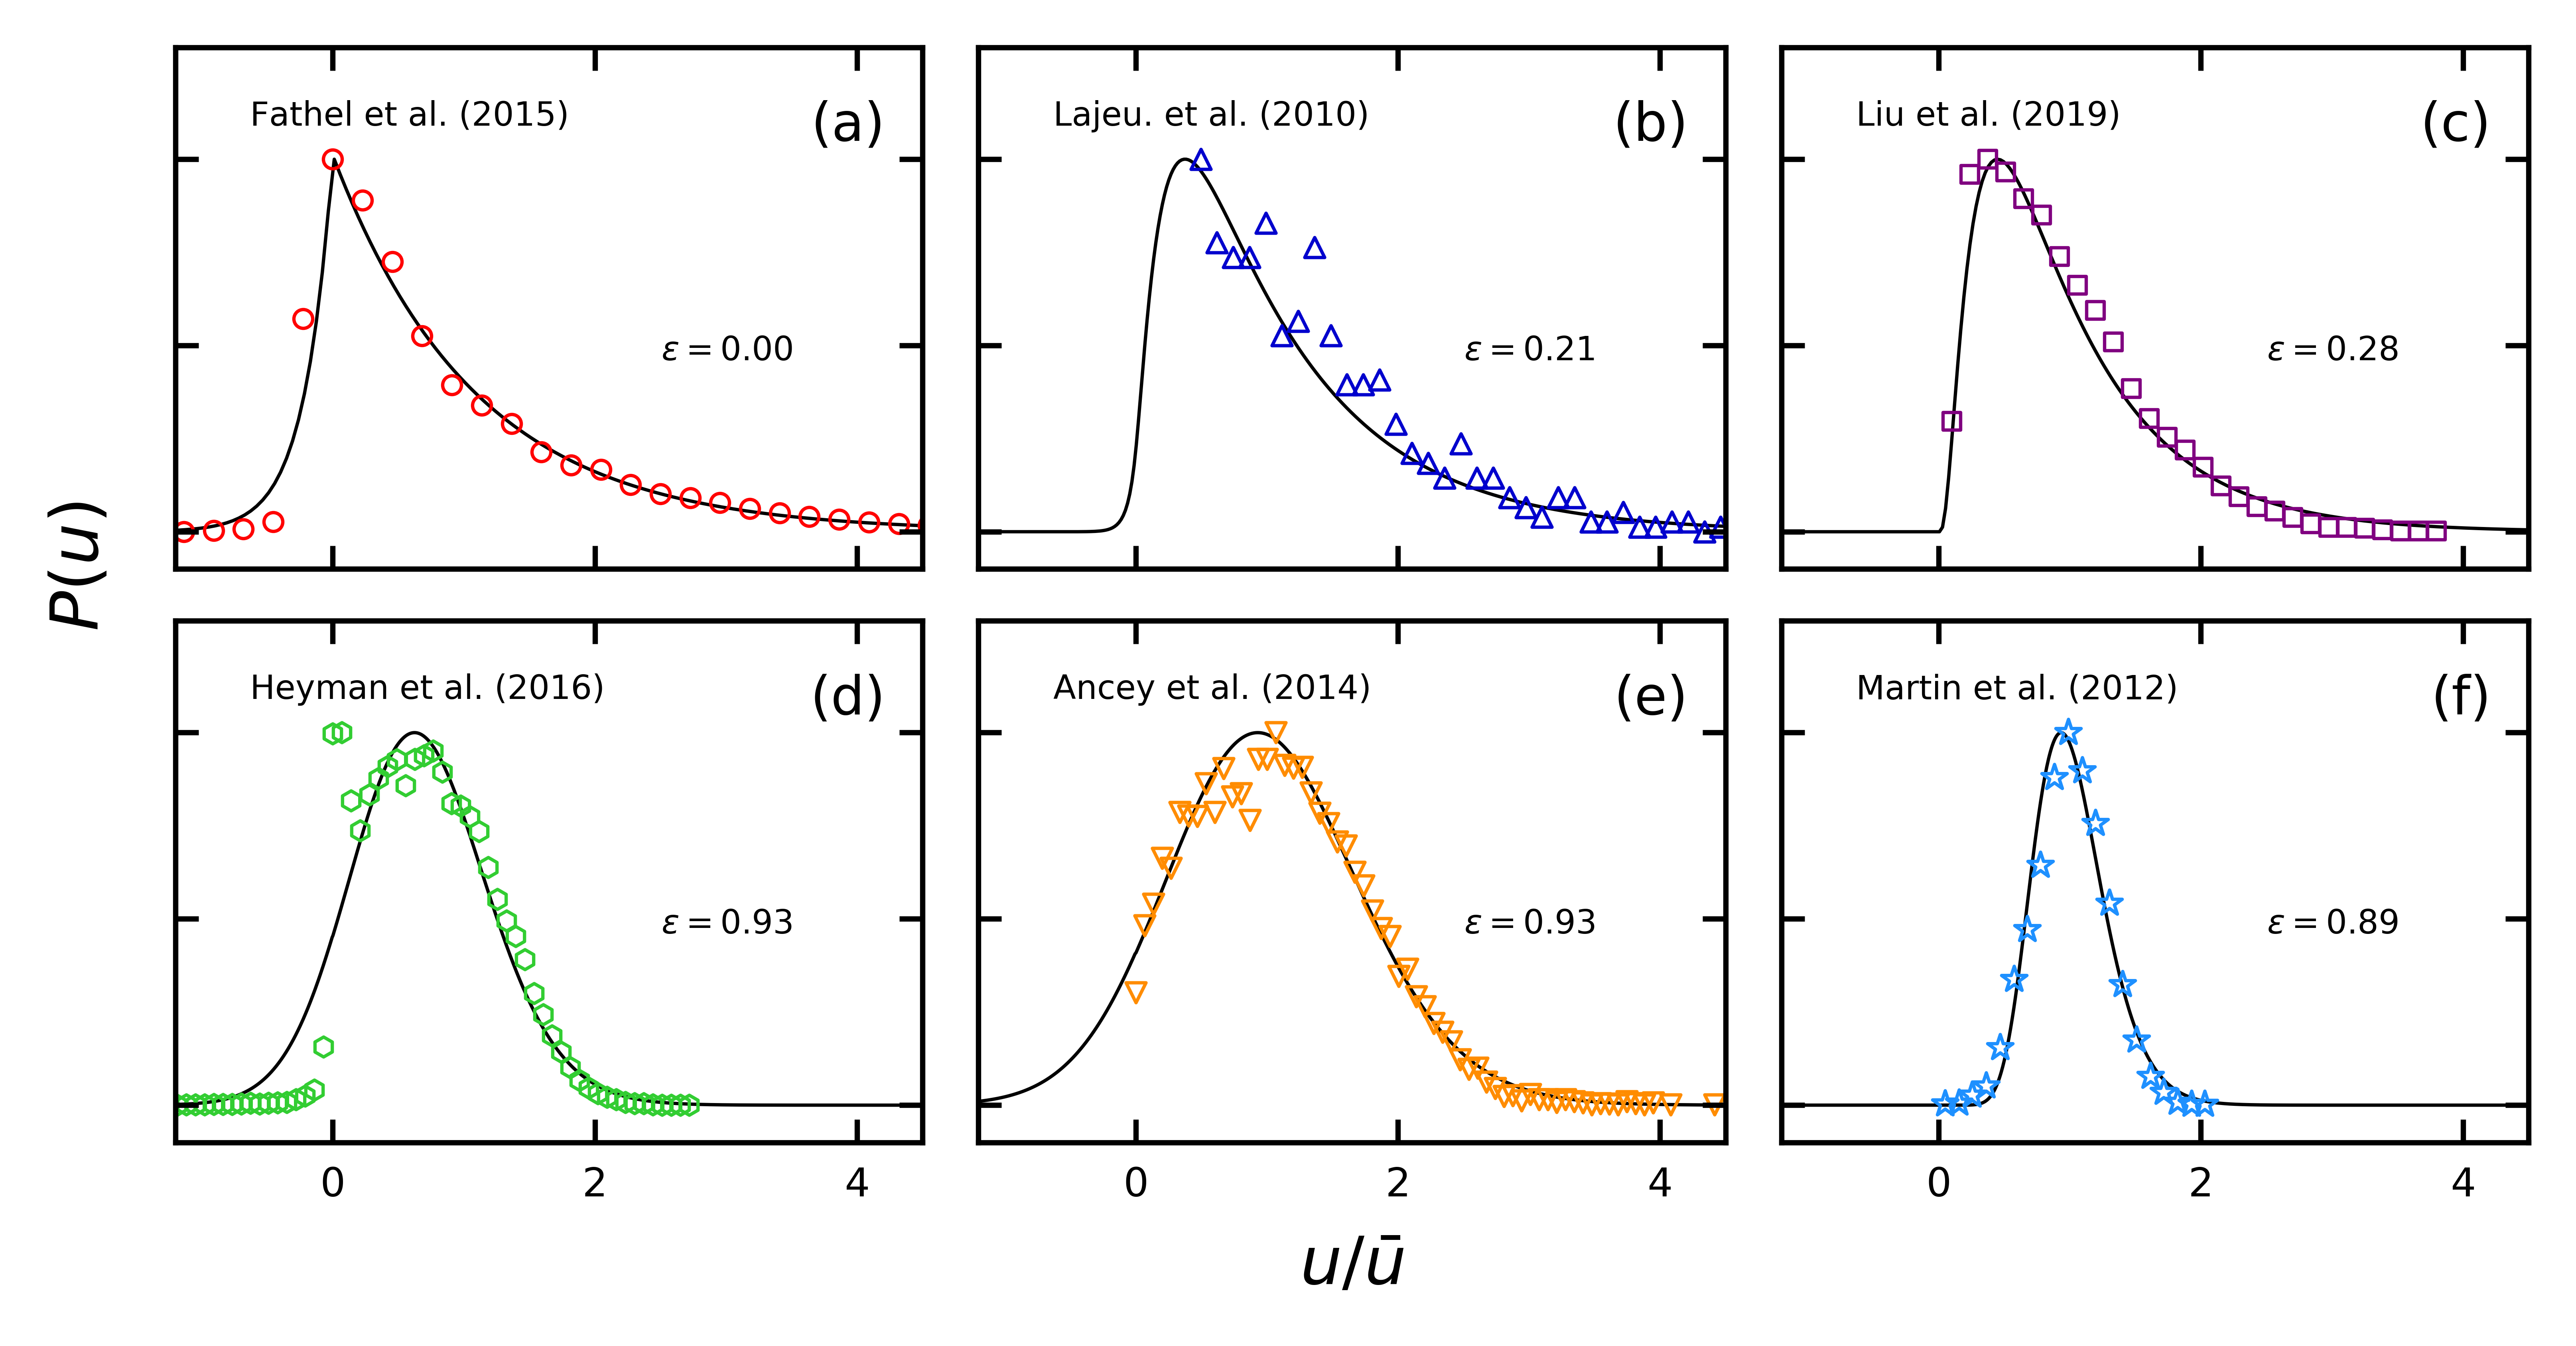
\includegraphics{./figures/ch5/Fig4expComparison.png}}
	\caption{The available experimental data on velocity distributions is compared to Eq. \ref{eq:steadystate} with calibration parameters $\nu$, $\varepsilon$, and $D$. In all cases there is good agreement, indicating that the model produces the range of distributions seen in the experimental data.} \label{fig:fig4ch5}
\end{figure}


\section{Discussion}
\label{sec:langdiscussion}

In this final chapter I developed a Langevin description of bedload sediment transport which includes episodic collisions between particles and the bed.
The model relates the shape of the instantaneous streamwise particle velocity distribution to the elasticity of particle-bed collisions.
This work generalizes earlier approaches available in the literature which did not include episodic collisions \citep{Ancey2014,Fan2014}, and provides a new physical explanation for the different streamwise sediment velocity distributions resolved in experiments.

Although in reality, the turbulent forces on moving sediment particles vary in a complex spatio-temporal way, I have approximated the fluid forces on bedload particles as spatially-uniform Gaussian white noise for reasons of analytical tractability \cite[e.g.][]{Michaelides1997}. Even though the non-Gaussian, space- and time-varying, and history-dependent aspects of fluid turbulence certainly do impact sediment movement \citep{Cameron2020,Celik2014}, this flow model appears more or less justified since sediment transport experiments provide similar velocity distributions regardless of whether the flow is laminar or turbulent \citep{Lajeunesse2010, Charru2004}, and since particle relaxation times are typically large compared to the timescales of turbulent fluctuations \citep{Hofland2006,Schmeeckle2007,Nakagawa1981}.
Nevertheless, it is possible that the vertical flow structure, and in particular the size of particles in comparison to the thickness of the laminar sub-layer, may be explanatory of the different velocity distributions resolved in bedload transport experiments, and future studies should investigate this possibility.

The model developed in this chapter described particle-bed collision forces as a sequence of instantaneous impulses in an approach that is reminiscent of the kinetic theory of gases \citep{Landau1969,Brilliantov2004}.
The effect of each collision on the streamwise particle velocity was described by a simple elasticity-like coefficient.
Although such approximate descriptions of particle-particle collisions are common in the theory of granular gases, the elasticity coefficient introduced here is not equivalent to the ``coefficient of restitution" typically applied in granular gas theory.
The coefficient of restitution is defined normal to the contact plane of two particles during a collision, and it characterizes energy loss due to deformation of the colliding particles in the absence of a viscous fluid \citep{Brach1992,Ismail2008}.

In bedload transport, colliding particles are submerged in a viscous fluid, and this introduces additional damping processes besides particle deformation \citep{Joseph2001,Yang2006,Schmeeckle2001}.
The model developed here does not consider these viscous forces, nor does it explicitly model the geometry of collisions, as $\ve$ was defined as a parameter applying to the downstream velocity only.
Thus, although I have included episodic particle-bed collisions in a stochastic sediment transport model for the first time, the key parameter $\ve$ in this formulation has a rather heuristic character and is not clearly related to the coefficient of restitution from granular gas theory.
Future studies should formulate particle-bed collisions in stochastic sediment transport models considering more details of collision geometry \citep{Sekine1992}, fluid-particle interactions \citep{Marshall2011}, and traditional restitution \citep{Brach1989} using the stochastic methods in the present study as a starting point. 

\subsection{Does the velocity distribution depend on particle size?}

Several researchers have considered why particle velocity distributions differ from one experiment to the next.
A prevailing view is that it relates to flow hydraulics \citep{Wu2020}. Many of the experiments producing Gaussian velocity distributions were conducted in supercritical flows \citep[e.g.][]{Heyman2016,Martin2012,Ancey2014}, whereas many producing exponential distributions were conducted in subcritical flows \citep[e.g.][]{Fathel2015,Charru2004,Seizilles2014}.
However several experiments run counter to this hypothesis.
The experiments of \citet{Lajeunesse2010} produced distinctly exponential velocity distributions in flows well within the supercritical regime ($\Fro=1.5$), whereas \citet{Liu2019} produced Gamma-like distributions in the subcritical regime ($\Fro=0.3$).

An alternative viewpoint, formulated in this chapter, is that the shape of the velocity distribution originates mainly from granular interactions.
Particle size enters the Langevin model Eq. \ref{eq:langevin} explicitly within the steady component of the drag, but it may also enter implicitly through the elasticity parameter $\ve$.
The analytical velocity distribution Eq. \ref{eq:steadystate} was fit to six different experimental datasets in Fig. \ref{fig:fig4ch5}, and the best fit parameters were presented in Tab. \ref{tab:calib}.
These fit parameters suggest collisions are generally less elastic for smaller particle sizes, whereas they are more elastic for larger particle sizes. This suggests that the amount of momentum dissipated by collisions may depend on particle size.

Because the elasticity $\ve$ lumps together collision geometry and dissipation effects, it is challenging to attribute the increasing relationship between elasticity and particle size evident in Tab. \ref{tab:calib} directly to particle size.
Yet this would be consistent with experiments of idealized particle collisions in viscous fluids. These demonstrate that momentum dissipation varies sharply with particle size, being more elastic for large particles, and less elastic for small particles \citep{Joseph2001,Yang2006,Schmeeckle2001}, exactly like the trend in the table.
A definite conclusion that particle size controls the shape of the bedload velocity distribution requires additional experimental and theoretical study. This work nevertheless produces suggestive ideas.

\section{Summary}
\label{sec:langconclusion}
This chapter has presented a Langevin description of individual bedload particles saltating downstream through episodic collisions.
The model suggests that episodic particle-bed collisions control the shape of the particle velocity distribution, and it is the first model to describe the range of bedload velocity distributions which have to date been reported in experimental studies.

This work suggests that particle-bed collisions may be a leading order control over the velocity distributions of bedload particles, although future study is required for a definite conclusion.
The next steps are to build up the episodic collision model presented in this chapter to include the geometric details of particle-bed collisions and to introduce slip velocity dependence and vertical structure into the flow forces acting on moving particles.
These efforts would produce additional insight into the controls of fluid turbulence and transverse, vertical, and rotational movements on the downstream velocities of individual bedload grains.

